\documentclass[]{article}
\usepackage{lmodern}
\usepackage{amssymb,amsmath}
\usepackage{ifxetex,ifluatex}
\usepackage{fixltx2e} % provides \textsubscript
\ifnum 0\ifxetex 1\fi\ifluatex 1\fi=0 % if pdftex
  \usepackage[T1]{fontenc}
  \usepackage[utf8]{inputenc}
\else % if luatex or xelatex
  \ifxetex
    \usepackage{mathspec}
  \else
    \usepackage{fontspec}
  \fi
  \defaultfontfeatures{Ligatures=TeX,Scale=MatchLowercase}
\fi
% use upquote if available, for straight quotes in verbatim environments
\IfFileExists{upquote.sty}{\usepackage{upquote}}{}
% use microtype if available
\IfFileExists{microtype.sty}{%
\usepackage[]{microtype}
\UseMicrotypeSet[protrusion]{basicmath} % disable protrusion for tt fonts
}{}
\PassOptionsToPackage{hyphens}{url} % url is loaded by hyperref
\usepackage[unicode=true]{hyperref}
\hypersetup{
            pdftitle={Empirical tuning rules according to Ziegler and Nichols},
            pdfkeywords={main},
            pdfborder={0 0 0},
            breaklinks=true}
\urlstyle{same}  % don't use monospace font for urls
\usepackage{longtable,booktabs}
% Fix footnotes in tables (requires footnote package)
\IfFileExists{footnote.sty}{\usepackage{footnote}\makesavenoteenv{long table}}{}
\usepackage{graphicx,grffile}
\makeatletter
\def\maxwidth{\ifdim\Gin@nat@width>\linewidth\linewidth\else\Gin@nat@width\fi}
\def\maxheight{\ifdim\Gin@nat@height>\textheight\textheight\else\Gin@nat@height\fi}
\makeatother
% Scale images if necessary, so that they will not overflow the page
% margins by default, and it is still possible to overwrite the defaults
% using explicit options in \includegraphics[width, height, ...]{}
\setkeys{Gin}{width=\maxwidth,height=\maxheight,keepaspectratio}
\IfFileExists{parskip.sty}{%
\usepackage{parskip}
}{% else
\setlength{\parindent}{0pt}
\setlength{\parskip}{6pt plus 2pt minus 1pt}
}
\setlength{\emergencystretch}{3em}  % prevent overfull lines
\providecommand{\tightlist}{%
  \setlength{\itemsep}{0pt}\setlength{\parskip}{0pt}}
\setcounter{secnumdepth}{0}
% Redefines (sub)paragraphs to behave more like sections
\ifx\paragraph\undefined\else
\let\oldparagraph\paragraph
\renewcommand{\paragraph}[1]{\oldparagraph{#1}\mbox{}}
\fi
\ifx\subparagraph\undefined\else
\let\oldsubparagraph\subparagraph
\renewcommand{\subparagraph}[1]{\oldsubparagraph{#1}\mbox{}}
\fi

% set default figure placement to htbp
\makeatletter
\def\fps@figure{htbp}
\makeatother


\title{Empirical tuning rules according to Ziegler and Nichols}
\date{}

\begin{document}
\maketitle

\href{http://www.atp.ruhr-uni-bochum.de/rt1/syscontrol/node65.html}{
\includegraphics[width=0.38542in,height=0.25000in]{./Empirical tuning rules according to Ziegler and Nichols_files/next.png}}
\href{http://www.atp.ruhr-uni-bochum.de/rt1/syscontrol/node60.html}{
\includegraphics[width=0.27083in,height=0.25000in]{./Empirical tuning rules according to Ziegler and Nichols_files/up.png}}
\href{http://www.atp.ruhr-uni-bochum.de/rt1/syscontrol/node63.html}{
\includegraphics[width=0.65625in,height=0.25000in]{./Empirical tuning rules according to Ziegler and Nichols_files/prev.png}}
\href{http://www.atp.ruhr-uni-bochum.de/rt1/syscontrol/node1.html}{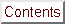
\includegraphics[width=0.67708in,height=0.25000in]{./Empirical tuning rules according to Ziegler and Nichols_files/contents.png}}\\
\textbf{Next:}
\href{http://www.atp.ruhr-uni-bochum.de/rt1/syscontrol/node65.html}{Design
of controllers using} \textbf{Up:}
\href{http://www.atp.ruhr-uni-bochum.de/rt1/syscontrol/node60.html}{PID
control and associated} \textbf{Previous:}
\href{http://www.atp.ruhr-uni-bochum.de/rt1/syscontrol/node63.html}{Advantages
and disadvantages of} ~
\textbf{\href{http://www.atp.ruhr-uni-bochum.de/rt1/syscontrol/node1.html}{Contents}}\\[2\baselineskip]

\section[ Empirical tuning rules according to Ziegler and
Nichols]{\texorpdfstring{\protect\hypertarget{SECTION00940000000000000000}{}{}
\protect\hypertarget{16224}{}{} \protect\hypertarget{16225}{}{}
\protect\hypertarget{16226}{}{}\protect\hypertarget{16227}{}{}
\protect\hypertarget{sec:empir-einst-nach8.2.3.1}{}{} Empirical tuning
rules according to Ziegler and
Nichols}{     Empirical tuning rules according to Ziegler and Nichols}}\label{empirical-tuning-rules-according-to-ziegler-and-nichols}

Many industrial processes show step responses with pure aperiodic
\protect\hypertarget{16229}{}{}behaviour according to
Figure~\href{http://www.atp.ruhr-uni-bochum.de/rt1/syscontrol/node64.html\#fig:8.2.7}{8.6}.
This S-shape curve is characteristic of many high-order systems and such
plant transfer functions may be approximated by the
\protect\hypertarget{16231}{}{}mathematical model

\protect\hypertarget{eq:8.2.32}{}{}

\begin{longtable}[]{@{}ll@{}}
\toprule
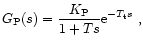
\includegraphics[width=1.48958in,height=0.46875in]{./Empirical tuning rules according to Ziegler and Nichols_files/img1239.png}
& (8.15)\tabularnewline
\bottomrule
\end{longtable}

which contains a 1st-order delay element and a
\protect\hypertarget{16239}{}{}dead time.
Figure~\href{http://www.atp.ruhr-uni-bochum.de/rt1/syscontrol/node64.html\#fig:8.2.7}{8.6}
shows the \protect\hypertarget{16438}{}{}approximation by a
\protect\hypertarget{16439}{}{}
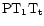
\includegraphics[width=0.45833in,height=0.27083in]{./Empirical tuning rules according to Ziegler and Nichols_files/img1241.png}
element.

\protect\hypertarget{fig:8.2.7}{}{}\protect\hypertarget{16440}{}{}

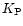
\includegraphics[width=0.23958in,height=0.27083in]{./Empirical tuning rules according to Ziegler and Nichols_files/img62.png}
(gain of the plant),
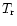
\includegraphics[width=0.17708in,height=0.27083in]{./Empirical tuning rules according to Ziegler and Nichols_files/img63.png}
(rise time) and
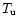
\includegraphics[width=0.18750in,height=0.27083in]{./Empirical tuning rules according to Ziegler and Nichols_files/img64.png}
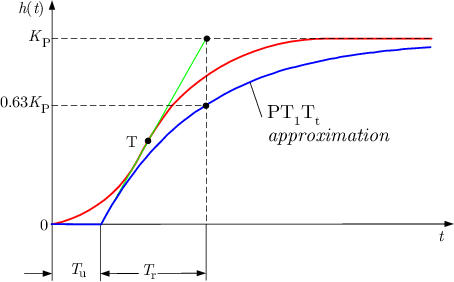
\includegraphics[width=4.72917in,height=2.93750in]{./Empirical tuning rules according to Ziegler and Nichols_files/img1242.png}


Here the step response is characterised by constructing the
\protect\hypertarget{16260}{}{}\protect\hypertarget{16261}{}{}tangent at
the turning point
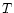
\includegraphics[width=0.14583in,height=0.13542in]{./Empirical tuning rules according to Ziegler and Nichols_files/img1243.png}
with the following three values:
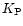
\includegraphics[width=0.23958in,height=0.27083in]{./Empirical tuning rules according to Ziegler and Nichols_files/img62.png}
(\protect\hypertarget{16263}{}{} \protect\hypertarget{16264}{}{}gain of
the plant),
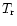
\includegraphics[width=0.17708in,height=0.27083in]{./Empirical tuning rules according to Ziegler and Nichols_files/img63.png}
\protect\hypertarget{16266}{}{} \protect\hypertarget{16267}{}{}(rise
time) and
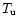
\includegraphics[width=0.18750in,height=0.27083in]{./Empirical tuning rules according to Ziegler and Nichols_files/img64.png}
\protect\hypertarget{16269}{}{} \protect\hypertarget{16270}{}{}(delay
time). Then a rough approximation according to
Eq.~(\href{http://www.atp.ruhr-uni-bochum.de/rt1/syscontrol/node64.html\#eq:8.2.32}{8.15})
is to set
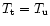
\includegraphics[width=0.52083in,height=0.27083in]{./Empirical tuning rules according to Ziegler and Nichols_files/img1244.png}
and
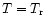
\includegraphics[width=0.46875in,height=0.27083in]{./Empirical tuning rules according to Ziegler and Nichols_files/img1245.png}.

For a plant of the type described above a lot of tuning rules for
standard controllers have been developed. These have been mostly
developed empirically from simulation studies. The most famous empirical
tuning rules are those of \emph{Ziegler} and \emph{Nichols}. These
tuning rules have been derived to provide step responses for the closed
loop, where the response shows a decrease of the amplitude of
approx.~25\% per period. For the application of these rules according to
Ziegler and Nichols two different approaches can be used:

\begin{description}
\item[a)]
\emph{\protect\hypertarget{16278}{}{}Method of the stability margin(I):}
Here, the following steps are used:

\begin{enumerate}
\tightlist
\item
  The controller is switched to pure P action.
\item
  The gain
  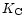
\includegraphics[width=0.25000in,height=0.27083in]{./Empirical tuning rules according to Ziegler and Nichols_files/img1108.png}
  of the P controller is continuously increased until the closed loop
  shows permanent oscillations. The value of the gain
  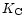
\includegraphics[width=0.25000in,height=0.27083in]{./Empirical tuning rules according to Ziegler and Nichols_files/img1108.png}
  at this state is denoted as the
  \protect\hypertarget{16282}{}{}\protect\hypertarget{16283}{}{}critical
  controller gain
  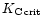
\includegraphics[width=0.44792in,height=0.27083in]{./Empirical tuning rules according to Ziegler and Nichols_files/img1246.png}.
\item
  The length of period
  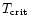
\includegraphics[width=0.30208in,height=0.27083in]{./Empirical tuning rules according to Ziegler and Nichols_files/img1247.png}
  \protect\hypertarget{16286}{}{}
  \protect\hypertarget{16287}{}{}(critical period) of the oscillations
  is measured.
\item
  From
  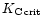
\includegraphics[width=0.44792in,height=0.27083in]{./Empirical tuning rules according to Ziegler and Nichols_files/img1246.png}
  and
  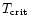
\includegraphics[width=0.30208in,height=0.27083in]{./Empirical tuning rules according to Ziegler and Nichols_files/img1247.png}
  one determines the controller tuning values
  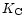
\includegraphics[width=0.25000in,height=0.27083in]{./Empirical tuning rules according to Ziegler and Nichols_files/img1108.png},
  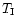
\includegraphics[width=0.16667in,height=0.27083in]{./Empirical tuning rules according to Ziegler and Nichols_files/img589.png}
  and
  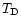
\includegraphics[width=0.21875in,height=0.27083in]{./Empirical tuning rules according to Ziegler and Nichols_files/img1193.png}
  using the formulas given in
  Table~\href{http://www.atp.ruhr-uni-bochum.de/rt1/syscontrol/node64.html\#tab:8.2.8}{8.1}.
\end{enumerate}
\item[b)]
\emph{\protect\hypertarget{16295}{}{}Method of the step response (II):}
In the case of an industrial plant it is often not possible, suitable or
allowed to drive the plant into \protect\hypertarget{16296}{}{}permanent
oscillations for determining
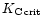
\includegraphics[width=0.44792in,height=0.27083in]{./Empirical tuning rules according to Ziegler and Nichols_files/img1246.png}
and
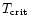
\includegraphics[width=0.30208in,height=0.27083in]{./Empirical tuning rules according to Ziegler and Nichols_files/img1247.png}.
Measuring the \protect\hypertarget{16299}{}{}step response of the plant
does not generally cause difficulties. Therefore, in many cases the
second form of the Ziegler-Nichols approach is more expedient. The rules
are based directly on the slope
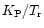
\includegraphics[width=0.45833in,height=0.29167in]{./Empirical tuning rules according to Ziegler and Nichols_files/img1248.png}
of the tangent at the turning point and on the delay
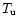
\includegraphics[width=0.18750in,height=0.27083in]{./Empirical tuning rules according to Ziegler and Nichols_files/img64.png}
of the step response. One has to observe that the measurement of the
step response needs only to be taken at the turning point T, as the
slope of the tangent already describes the ratio
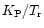
\includegraphics[width=0.45833in,height=0.29167in]{./Empirical tuning rules according to Ziegler and Nichols_files/img1248.png}.
Using the measured data
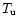
\includegraphics[width=0.18750in,height=0.27083in]{./Empirical tuning rules according to Ziegler and Nichols_files/img64.png}
and
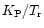
\includegraphics[width=0.45833in,height=0.29167in]{./Empirical tuning rules according to Ziegler and Nichols_files/img1248.png}
as well as the formula given in
Table~\href{http://www.atp.ruhr-uni-bochum.de/rt1/syscontrol/node64.html\#tab:8.2.8}{8.1}
the controller tuning parameters can be determined by simple
calculations.
\end{description}

\protect\hypertarget{16311}{}{}

\begin{longtable}[]{@{}l@{}}
\caption{\textbf{Table 8.1:} Controller tuning parameters according to
Ziegler and Nichols}\tabularnewline
\toprule
\begin{minipage}[t]{0.97\columnwidth}\raggedright\strut
\protect\hypertarget{tab:8.2.8}{}{}
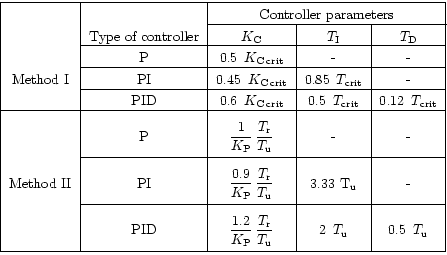
\includegraphics[width=4.65625in,height=2.65625in]{./Empirical tuning rules according to Ziegler and Nichols_files/img1249.png}\strut
\end{minipage}\tabularnewline
\bottomrule
\end{longtable}

\textbf{Demonstration Example 8.1} ~ \protect\hypertarget{16364}{}{}
\protect\hypertarget{zieglernicholsexample}{}{}
\href{http://virtual.cvut.cz/virtualexperiments/optocon.html}{A virtual
experiment using PID control for tracking}

\textbf{Demonstration Example 8.2} ~ \protect\hypertarget{16370}{}{}
\protect\hypertarget{zieglernicholsexample2}{}{}
\href{http://virtual.cvut.cz/virtualexperiments/hydraulic.html}{A
virtual experiment using PID control for high-precision positioning}

\textbf{DYNAST study example 8.1} ~ \protect\hypertarget{16376}{}{}
\protect\hypertarget{PIPT1tt}{}{}
\href{http://virtual.cvut.cz/dyn/examples/examples/control/ac3pid1/index.html}{PI
control of a PT\textsubscript{1}T\textsubscript{t} plant}

\textbf{DYNAST study example 8.2} ~ \protect\hypertarget{16382}{}{}
\protect\hypertarget{PIDPT1tt}{}{}
\href{http://virtual.cvut.cz/dyn/examples/examples/control/ac3pid2/index.html}{PID
control of a PT\textsubscript{1}T\textsubscript{t} plant}

\textbf{DYNAST study example 8.3} ~ \protect\hypertarget{16388}{}{}
\protect\hypertarget{DisturbancePIPT1tt}{}{}\href{http://virtual.cvut.cz/dyn/examples/examples/control/ac8distpi/index.html}{Disturbance
response for PI control of a PT\textsubscript{1}T\textsubscript{t}
plant}

\begin{center}\rule{0.5\linewidth}{\linethickness}\end{center}

\href{http://www.atp.ruhr-uni-bochum.de/rt1/syscontrol/node65.html}{
\includegraphics[width=0.38542in,height=0.25000in]{./Empirical tuning rules according to Ziegler and Nichols_files/next.png}}
\href{http://www.atp.ruhr-uni-bochum.de/rt1/syscontrol/node60.html}{
\includegraphics[width=0.27083in,height=0.25000in]{./Empirical tuning rules according to Ziegler and Nichols_files/up.png}}
\href{http://www.atp.ruhr-uni-bochum.de/rt1/syscontrol/node63.html}{
\includegraphics[width=0.65625in,height=0.25000in]{./Empirical tuning rules according to Ziegler and Nichols_files/prev.png}}
\href{http://www.atp.ruhr-uni-bochum.de/rt1/syscontrol/node1.html}{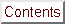
\includegraphics[width=0.67708in,height=0.25000in]{./Empirical tuning rules according to Ziegler and Nichols_files/contents.png}}\\
\textbf{Next:}
\href{http://www.atp.ruhr-uni-bochum.de/rt1/syscontrol/node65.html}{Design
of controllers using} \textbf{Up:}
\href{http://www.atp.ruhr-uni-bochum.de/rt1/syscontrol/node60.html}{PID
control and associated} \textbf{Previous:}
\href{http://www.atp.ruhr-uni-bochum.de/rt1/syscontrol/node63.html}{Advantages
and disadvantages of} ~
\textbf{\href{http://www.atp.ruhr-uni-bochum.de/rt1/syscontrol/node1.html}{Contents}}

Christian~Schmid~2005-05-09

\end{document}
